\documentclass[12pt,]{report}
\usepackage{lmodern}
\usepackage{amssymb,amsmath}
\usepackage{ifxetex,ifluatex}
\usepackage{fixltx2e} % provides \textsubscript
\ifnum 0\ifxetex 1\fi\ifluatex 1\fi=0 % if pdftex
  \usepackage[T1]{fontenc}
  \usepackage[utf8]{inputenc}
\else % if luatex or xelatex
  \ifxetex
    \usepackage{mathspec}
  \else
    \usepackage{fontspec}
  \fi
  \defaultfontfeatures{Ligatures=TeX,Scale=MatchLowercase}
    \setmainfont[]{Helvetica}
    \setsansfont[]{Helvetica}
    \setmonofont[Mapping=tex-ansi]{Helvetica}
\fi
% use upquote if available, for straight quotes in verbatim environments
\IfFileExists{upquote.sty}{\usepackage{upquote}}{}
% use microtype if available
\IfFileExists{microtype.sty}{%
\usepackage{microtype}
\UseMicrotypeSet[protrusion]{basicmath} % disable protrusion for tt fonts
}{}
\usepackage[margin=1in]{geometry}
\usepackage{hyperref}
\hypersetup{unicode=true,
            pdftitle={Characterisation of model species interactome available from primary molecular interaction databases},
            pdfauthor={Vitalii Kleshchevnikov},
            pdfborder={0 0 0},
            breaklinks=true}
\urlstyle{same}  % don't use monospace font for urls
\usepackage{natbib}
\bibliographystyle{plainnat}
\usepackage{graphicx,grffile}
\makeatletter
\def\maxwidth{\ifdim\Gin@nat@width>\linewidth\linewidth\else\Gin@nat@width\fi}
\def\maxheight{\ifdim\Gin@nat@height>\textheight\textheight\else\Gin@nat@height\fi}
\makeatother
% Scale images if necessary, so that they will not overflow the page
% margins by default, and it is still possible to overwrite the defaults
% using explicit options in \includegraphics[width, height, ...]{}
\setkeys{Gin}{width=\maxwidth,height=\maxheight,keepaspectratio}
\IfFileExists{parskip.sty}{%
\usepackage{parskip}
}{% else
\setlength{\parindent}{0pt}
\setlength{\parskip}{6pt plus 2pt minus 1pt}
}
\setlength{\emergencystretch}{3em}  % prevent overfull lines
\providecommand{\tightlist}{%
  \setlength{\itemsep}{0pt}\setlength{\parskip}{0pt}}
\setcounter{secnumdepth}{0}
% Redefines (sub)paragraphs to behave more like sections
\ifx\paragraph\undefined\else
\let\oldparagraph\paragraph
\renewcommand{\paragraph}[1]{\oldparagraph{#1}\mbox{}}
\fi
\ifx\subparagraph\undefined\else
\let\oldsubparagraph\subparagraph
\renewcommand{\subparagraph}[1]{\oldsubparagraph{#1}\mbox{}}
\fi

%%% Use protect on footnotes to avoid problems with footnotes in titles
\let\rmarkdownfootnote\footnote%
\def\footnote{\protect\rmarkdownfootnote}

%%% Change title format to be more compact
\usepackage{titling}

% Create subtitle command for use in maketitle
\newcommand{\subtitle}[1]{
  \posttitle{
    \begin{center}\large#1\end{center}
    }
}

\setlength{\droptitle}{-2em}
  \title{Characterisation of model species interactome available from primary
molecular interaction databases}
  \pretitle{\vspace{\droptitle}\centering\huge}
  \posttitle{\par}
  \author{Vitalii Kleshchevnikov}
  \preauthor{\centering\large\emph}
  \postauthor{\par}
  \predate{\centering\large\emph}
  \postdate{\par}
  \date{21 December 2016}


\begin{document}
\maketitle

{
\setcounter{tocdepth}{1}
\tableofcontents
}
The report was published on 2017-09-25. Data used in the report was
available on 2017-09-25.

\chapter{Outline}\label{outline}

\begin{enumerate}
\def\labelenumi{\arabic{enumi}.}
\tightlist
\item
  Abstract
\item
  Introduction
\item
  Methods
\item
  Results and discussion

  \begin{itemize}
  \tightlist
  \item
    how available interactome covers the proteome
  \item
    IntAct(IMEx) vs Biogrid
  \item
    which proteins are missing
  \item
    interaction detection biases
  \item
    study bias: the more articles, the more interactions
  \item
    which protein function are interaction databases and high-throughput
    datasets enriched in?
  \end{itemize}
\item
  Conclusion
\end{enumerate}

\chapter{Abstract}\label{abstract}

The structure and the function of the cell arise from interactions
between molecules inside and outside it. Investigation of those
interactions is, therefore, necessary (but not sufficient) to obtain the
understanding of the living systems. Gathering interaction data and
depositing it in a central database for open and easy access by the
research community can and does accelerate progress in the field. An
attempt to unify interaction data from multiple sources meets many
challenges, such as standardisation of annotation, interoperability with
other resources and time it takes to manually gather the data. As new
network analysis methods become available and research group start to
use molecular interaction data to make inferences, generate new
hypotheses and explain the results of transcriptomics and proteomics the
coverage of the real interactome by our knowledge and the bias present
in the databases begin to influence research results. This motivates the
need to identify which proteins have no interactions are available and
understand biases in our interaction data. We focus our analysis on the
data deposited to the IMEx consortium of primary databases, which
includes the IntAct database, the resource supported by our group.

The best coverage we observe is for yeast, \emph{E.coli} and human.
Isoform coverage is limited, but still significant for human.\\
We have investigated if IntAct database coverage is biased towards
physicochemical properties of the protein and how well described the
protein is in the literature. Proteins with no interactions in IntAct
are on average smaller, less well-studied overall, have a lower fraction
of charged residues and higher mean hydropathy. Next, we have
investigated if two high-throughput interaction detection methods (which
use distinct strategies) may be biased towards physicochemical
properties of the protein (such as mass): AP-MS and two-hybrid. Affinity
purification followed by mass spectrometry (AP-MS) seems to capture a
higher proportion of larger proteins as compared to two-hybrid methods.
By performing enrichment analysis of the molecular function (Gene
Ontology) we have found that databases and datasets which contain
experimentally derived data are enriched and depleted in the same
functional categories. STRING database, which includes computational
prediction data, is the least biased.\\
These results can inform literature curation by IMEx consortium teams
and data integration efforts.

\chapter{Introduction}\label{introduction}

The structure and the function of the cell arise from interactions
between molecules inside and outside it \citep{Hein:2015aa}. Though
proteins, nucleic acids, lipids and small molecules can all form
important interactions, studies and literature focus mainly on
interactions between proteins and other macromolecules. We can discover
and study these molecular interactions using a number of experimental
and computational techniques. This study aims to describe the coverage
and the biases of currently available molecular interaction data. We
focus on molecular interactions identified in the experimental setting
most of which are represented (in the literature and databases) by
protein-protein interactions (although, there is a considerable amount
of data on protein-DNA interactions, for example, ChIP-Seq data, which
is traditionally incorporated into the genomic or specialist databases).
We focus on specifically on protein-protein interaction data.

Molecular interactions can be classified using multiple criteria: the
information interaction detection methods can provide towards ground
truth, interaction detection method, biological role of the interaction
(covalent binding, enzymatic reaction, e.g.) which can be explored in
molecular interaction ontology
\citep[\url{http://www.ebi.ac.uk/ols/ontologies/mi/}]{Hermjakob:2004aa}.
A standard way of describing interaction allows record published
interactions into databases, assign interactions a score based on the
evidence and reliability and, least but not last, reuse interaction data
for computational analyses, gaining insight into the novel fucntion of
proteins and generate hypothesis. In the recent years, the fact that
biases in molecular interaction data can mislead network-driven studies
has become evident \citep{Schaefer:2015aa}, which motivates the need to
study the coverage and bias of currectly available molecular interaction
data, identify missing proteins and molecular functions those protiens
perform. These results may help in selecting appropriate network data
for data integration studies.

We investigate the data in the IntAct database \citep{Orchard:2014aa}
which is provider of high-depth manually curated molecular interaction
data, a part of IMEx consortium. The IMEx consortium
\citep{Orchard:2012aa} is an international collaboration between a group
of major public interaction data providers who share curation effort.
This study can aid literature curation effort by IntAct group by
pointing to the publications contating interaction data on proteins with
no interactions currently deposited in the IntAct database.

\subsection{Defining interactome}\label{defining-interactome}

The aggregation of all components and their interactions into a single
network results in what we call interactome, the whole of all molecular
interactions. You can also look into the subset of this network, for
example, you can select only those proteins that are expressed in the
brain, and only the interactions between these proteins identified
experimentally in the brain cells. This example reflects the complexity
and the diversity of the interactome - which is what you would expect
from a system underlying the complexity and the diversity of the cell
types, cellular behaviours, and functions. For the same reason, only by
studying these interactions and how they change in specific cell types
and under specific circumstances in combination with the functional
analysis we can decipher cellular regulatory networks. The ultimate goal
of the research in the field would be to capture all physical
interactions and thoroughly describe them while avoiding false positive
results.

\subsection{Experimental approaches for discovering
interactions}\label{experimental-approaches-for-discovering-interactions}

\begin{figure}
\centering
\includegraphics{./Data/expansion_methods.png}
\caption{Figure 1. Association and physical associations identified
using AP-MS approaches fundamentally don't provide binary interactions.
Binary interactions have to be inferred from the list of proteins
represented as cluster on the left. Matrix expansion links every protein
to every other protein in the AP-MS-derived cluster. Spoke expansion
only links the bait with all other proteins in a cluster. As you can
see, none of these methods generate the exact set of binary interactions
that occur in reality. Spoke expansion tends to generate less
false-positives and is used more often.}
\end{figure}

Numerous experimental protein interaction detection methods are
currently widely used. The classification we provide is far from
comprehensive but gives a short description of the methods analysed in
this study. Based on the evidence provided and possibility to scale up
to high-throughput studies methods can be classified into 3 main
categories.\\
The first category is formed by methods using affinity purification to
capture all proteins associated with the bait. Only proteins that have a
direct or indirect physical connection with the bait will be purified.
Following purification procedure, those proteins can be identified using
western-blotting and specific antibody staining or using
mass-spectrometry, latter can be done in a high-throughput manner. The
main advantage of these methods is the potential ability capture any
protein, in different cellular contexts and to quantitatively
characterise interaction properties \citep{Hein:2015aa}. The main
disadvantage of these techniques comes from the fact that experiments
indentify both direct and indirect interactions between the bait and
captured proteins and no way of distinguishing those (although, one may
delete identified proteins one by one from the cell and decipher direct
interactions). This type of interactions in called associations and do
be represented in the network requires the use of expansion methods
(Figure 1, adopted from the IntAct website). The other drawback of this
method is dependency on the availability and quaility of antibodies for
affinity-purification step. We will call these methods
affinity-purification followed mass-spectrometry (AP-MS) across this
report.\\
As defined by molecular interaction ontology
\citep[\url{http://www.ebi.ac.uk/ols/ontologies/mi/}]{Hermjakob:2004aa},
an association is an interaction between molecules that may participate
in formation of one, but possibly more, physical complexes, association
will be called physical if experiments show enough evidence that
proteins are in the same physical complex but don't show direct
interaction.\\
The second category of methods is formed by protein complementation
techniques which include two-hybrid (transcription factor
complementation), the most widely used interaction detection method
(including high-throughput experiments). In this method, pairs of
proteins are tested for interaction and therefore discovered
interactions are more likely to be direct (the main advantage of this
method). Classic implementation of two-hybrid is performed in yeast
cells and requires studied proteins to be non-membrane, however,
two-hybrid for membrane proteins and for mammalian cells was also
developed \citep[\citet{Saraon:2017aa}]{Lemmens:2015aa}. The main
disadvantage of two-hybrid methods is that every protein has to be
cloned into a plasmid or other vector and exogenously expressed. Ability
to clone protein-coding sequence and, in case of yeast two-hybrid,
correct protein folding, are the limiting factors for two-hybrid but not
AP-MS techniques. As a side note, the lack of antibodies for a specific
bait protein may force researches to tag, clone and express protein
which is a subject to similar problems, however, AP-MS would allow
identification of the binding partners, no cloning needed.\\
Final category is formed by structure-based methods (co-crystallisation
and X-ray crystallography, e.g.). These methods can provide valuable
information on how exactly physical interaction occurs, however, these
methods are extremely labor-intensive and, therefore, non-scalable and
will always need complementary experiments showing if the proteins
actually interact in the cellular context.\\
To conclude, all protein interaction detection methods have their
strengts and weaknesses, so it is important to accept that every protein
interaction detection method has it's limitations in the ability to
identify true physical interaction and serves as evidence we use to
infer protein interaction. By combining different methods to identify
protein interaction we can gain more confidence in our findings and by
disrupting interaction under specific cellular context we can identify
it's function.

\subsection{Challenges of
interactomics}\label{challenges-of-interactomics}

Four big challenges substantially complicate the study of molecular
interactions, especially on the whole organism scale. The first being
that we don't know the true nature of underlying our experimental
results (all assays provide evidence that interaction is possible and
some can provide quantitative description, but all are prone to error
and the problem described in the figure 1 A) which lead to the necessity
of combining interaction data from multiple experiments and complex
statistical evaluation of how probable the interaction is based on that
data (such as Bayesian approach, \citet{Braun:2009aa},
\citet{Zhang:2011aa}) rather than receiving confident yes-or-no result
from a single experiment. Interaction databases make an effort to score
the interactions based on supporting evidence, however, this is usually
done with non-probabilistic heuristic approaches, such as MI score
implemented in IntAct \citep{Villaveces:2015aa}. Every database that
aggregates interaction data from other resources will develop an
algorithm to score interactions. The challenge is to identify when to
put the threshold betweem high and low confidence interactions or when
to say ``I am confident the interaction exists''.

The second big challenge is the problem of ``noise'' - or the problem of
false positives. Different interaction detection experiments are prone
to these errors for different reasons, for example, in-vitro experiments
(e.g.~TAP-MS) may allow the interaction between proteins which are
normally separated between different cellular compartments. Specific
groups of proteins (based on their physical or chemical properties,
abundance) may have a higher susceptibility to false positives, for
example, highly abundant proteins are easier to detect and may also be
less efficiently diluted during the affinity purification procedure,
which may lead to artifactual results. Contamination is another common
problem for AP-MS experiments which have motivated the creation of
contaminant database, CRAPOME \citep{Mellacheruvu:2013aa}. A more
general problem of noise can be addressed by proteome-scale
interactomics experiments (which can include enough samples to guarantee
low false positive rate while still identifying interactions).

The third big challenge is that our knowledge of interactome is
incomplete which arises from the fact that experimental approaches have
low statistical power and often miss out some real interactions. Many
efforts to reproduce protein interactions find little overlap between
the new and the original study \citep{Braun:2009aa}. Also, many
proteins, especially in non-model species have no know interactions.

The final challenge contributes to the ``incomplete interactome''
problem but is grounded in the fact that not all protein interaction
discovered and published are included in protein interaction databases.
In the other words, this is database curation problem. More than 100
public databases containing protein interactions are available now
{[}\url{http://pathguide.org/}{]}. These databases differ:\\
- by the types of data they include (e.g.~computational prediction,
manual curation experimental data from research papers (primary
databases), aggregated data from many primary databases (secondary
databases)),\\
- the level of detail captured from articles to describe interactions\\
- how often and if databases are updated with new data, identifiers and
annotation.\\
The level of detail ranges from mentioning only the pairs of interacting
partners and heuristic scores assigned to them (for instance, STRING) to
the ones containing experiment details (detection method, bait/prey
status, if available - quantitative data, experiment setup, protein
variants), such as IntAct \citep{Orchard:2014aa}.\\
The amount of interaction data generated per year is growing
exponentially making manual curation of all this data into primary
databases a daunting task. To prioritise curation efforts and reduce
redundancy between databases (to curate different data using the same
standards) IMEx consortium was formed in 2012 \citep{Orchard:2012aa}.
IMEx-compliant databases include primary databases such as IntAct and
MINT, but doesn't include BioGRID (which curates at the lower level of
detail) and no longer active databases such as HPRD \citep{Peri:2004aa}
and BIND \citep{Isserlin:2011aa}.

\chapter{Motivation for this study}\label{motivation-for-this-study}

Solving some of these challenges may be easier than the others. In
particular, to solve the last challenge we can prioritise curation
efforts for already published interactions to cover unrepresented
proteins and we can encourage authors to submit their results to the
databases prior to publishing. We can also encourage research of
underrepresented parts of the interactome. This motivates the need to
characterise the interactome already present in interaction databases.
More specifically, we need to measure how available interactome covers
the proteome of main model species, if there are any biases towards
proteins with or without available interactions and if major protein
interaction detection methods exhibit biases towards specific groups of
proteins. These results can be also used to inform data integration
projects and show the need to adjust for biases when studying
protein-protein interactions network.

\chapter{Aims of the study}\label{aims-of-the-study}

\begin{enumerate}
\def\labelenumi{\arabic{enumi}.}
\item
  Describe the coverage of the proteome of main model species.
  Considering either all UniProtKB or SwissProt entries only as the
  proteome (canonical identifiers as well as protein isoforms). Consider
  all interactions from IMEx-compliant databases as interactome.
\item
  Compare the coverage of the proteome by interaction evidence from IMEx
  to the interaction evidence from BioGRID (the other major primary
  database).
\item
  Investigate if proteins with no available interactions stand out by
  specific functions (Gene Ontology, GO: biological process and
  molecular function), cellular localisation (GO), molecular mass, or
  protein evidence status from SwissProt
\item
  Find out if major protein interaction detection methods (two-hybrid
  and AP-MS) exhibit any bias towards biochemical properties of the
  proteins involved (mass, disordered regions, hydropathy, the fraction
  of charged residues)
\end{enumerate}

\chapter{Methods: data processing and
analysis}\label{methods-data-processing-and-analysis}

\subsection{Getting proteome from
UniProtKB}\label{getting-proteome-from-uniprotkb}

Whole proteome (all UniProtKB) for each species was downloaded
programmatically in R using UniProt rest API. SwissProt-proteome was
subset from the whole proteome by reviewed status column. UniProt
identifies proteins by UniProtKB/AC (e.g.~P04637, accession) which does
not distinguish between protein isoforms. UniProt aggregates isoform
information and identifiers (e.g.~P04637-4) in a separate column with
zero to many isoforms per each UniProtKB accession. To generate proteome
list which includes protein isoforms, isoform accessions were extracted
and combined with the list of generic accessions. In this analysis,
protein evidence status and protein mass are only attributed to generic
accessions.

\subsection{Getting and transforming interactome data from IMEx
databases and
BioGRID}\label{getting-and-transforming-interactome-data-from-imex-databases-and-biogrid}

Interactome from all IMEx databases was downloaded programmatically in R
using PSIQUIC package from Bioconductor \citep{PSICQUIC}. The list of
interactions (pairs of interactors) was transformed into the list of
interactors preserving interactor identifiers, the type of interactor
identifier, species information and the database interaction originates
from. Only unique proteins wereIMEx databases contain interactions
between proteins, RNA, DNA and small molecules, moreover, these
interaction may involve molecules originating from different species.
Therefore, to perform by species interactome/proteome comparison there
is a need to remove non-UniProtKB/AC molecule identifiers (which removes
non-protein molecules, although, may also remove a small fraction of
proteins which have no UniProtKB/AC) and there is a need to remove
proteins originating from other species. Also, entries in IMEx databases
has to be cleaned of tags and textual descriptions
(``taxid:9606(human-h1299)\textbar{}taxid:9606(Homo sapiens lung lymph
node carcinoma)'' to ``9606'') to make further analysis easier and
cleaner. Next, when provided in the research articles protein isoform
information is always included in IMEx databases, so to perform analysis
excluding isoform information UniProtKB/AC were cleaned of -N suffix
(P04637-4 to P04637). IMEx consortium databases such as IntAct, MINT,
BHF-UCL, MPIDB, MatrixDB, HPIDb, I2D-IMEx, InnateDB-IMEx, MolCon,
UniProt, MBInfo are currently integrated into IntAct
\citep{Orchard:2014aa}. Data from all these databases was used in the
analysis and reffered to as IntAct data or IMEx data.

\subsection{Physicochemical properties and disordered region
prediction}\label{physicochemical-properties-and-disordered-region-prediction}

Information on disordered region content and physicochemical properties
of individual proteins were obtained from the dataset generated by
Vincent and Schnell in 2015 \citep{Vincent:2016aa}. Briefly, Vincent and
Schnell used a number of disorder prediction algorithms (IUPred and
DisEMBL) and their consensus to generate disordered region predictions
for each protein which was be used to calculate the fraction of
disordered regions in a protein. In addition, Vincent and Schnell used
localCIDER version 0.1.7 (Classification of Intrinsically Disordered
Ensemble Regions) to calculate physical properties such as fraction of
charged residues, mean hydropathy or charge separation for each protein.
This was done for 10 eukaryotic proteomes and written to SQLite-database
which was made available online through dryad service
\citep{dryad_sm107}.

\subsection{Gene Ontology enrichment
analysis}\label{gene-ontology-enrichment-analysis}

Enrichment analysis can identify groups of genes seletively enriched or
depleted in a specific dataset. Genes can be grouped by common
annotations decribing their function, location in the cell or membership
in a pathway, such as those described in KEGG \citep{Kanehisa:2016aa} or
Reactome \citep{Fabregat:2016aa}. Gene Ontology Consortium (GO)
\citep{Gene-Ontology:2015aa} annotates gene products (proteins,
non-coding RNA, protein complexes) by molecular fuction they perform,
cellular component they are located in and biological process they are
involved in. This annotation is first done manually by a curator based
on evidence provided in the research paper and then expanded to other
proteins using computational annotation methods, for example, mouse
orthologues of human protein are likely to have similar function.
Computational annotation is less reliable however it allows to generate
at annotations for non-studied proteins or in poorely studied organisms.
More information on the evidence codes for Gene Ontology annotations can
be found on the GO Consortium website
{[}\url{http://geneontology.org/page/guide-go-evidence-codes}{]}. All
analyses in this study included all Gene Ontology annotations.\\
Enrichment analysis uses statistical tests and protein to GO term
associations to identify functions and compartments overrepresented in a
particular list of proteins as compared to background list. Statistical
test is performed for every GO term and uses hypergeometric distubution
to estimate the probability that a number of proteins in our list is
annotated by a speficic GO term by chance based on the fraction of
proteins annotated with that term in the background list. Calculated
probality tells how likely (by chance) is that our list is enriched in
proteins with function described by that specific GO term. If that's
highly unlikely to occur by chance we consider GO function to be
enriched. Multiple hypothesis testing correction is applied to adjust
probabilies for higher probability of getting extreme result by chance
due to testing thousands of GO terms. All enrichment test were performed
and visualised using R package clusterProfiler \citep{Yu:2012aa}. GO
annotations used in the clusterProfiler package are compiled from GO
consortium into R package GO.db \citep{GO.db} provided through
Bioconductor project \citep{Gentleman:2004aa}.

\subsection{Computational analysis:
code}\label{computational-analysis-code}

All R code used in this analysis in deposited to a public Github
repository \citep{VKleshchevnikov2017}, which is a common code-sharing
resource.

\chapter{Results}\label{results}

\section{1. How well available interactome covers the
proteome}\label{how-well-available-interactome-covers-the-proteome}

\subsection{Available interactome covers substantial fraction of the
reviewed proteome of main model
species}\label{available-interactome-covers-substantial-fraction-of-the-reviewed-proteome-of-main-model-species}

In this section, we compare the proteome, the list of all proteins in
annotated Uniprot \citep{The-UniProt:2017aa}, to the list of proteins
which have interacting partners annotated in IMEx consortium databases.
We compare the coverage across seven model species. We have also
compared interactome coverage of the manually reviewed SwissProt (shown
on the Figure 7.1) and the reviewed SwissProt and unreviewed trEMBL (all
UniProtKB) combined shown on the Supplementary Figure 1.\\
Non-canonical protein isoform identifiers (P32054-1) were converted to
canonical identifiers (P32054) resulting in interactions ``any isoform
to any isoform'' (Venn diagrams on the right) or isoform identifiers
were preserved (Venn diagrams on the left). You can see that adding
isoform information adds more proteins to the SwissProt list but not so
many proteins to the IMEx list.

\begin{figure}
\centering
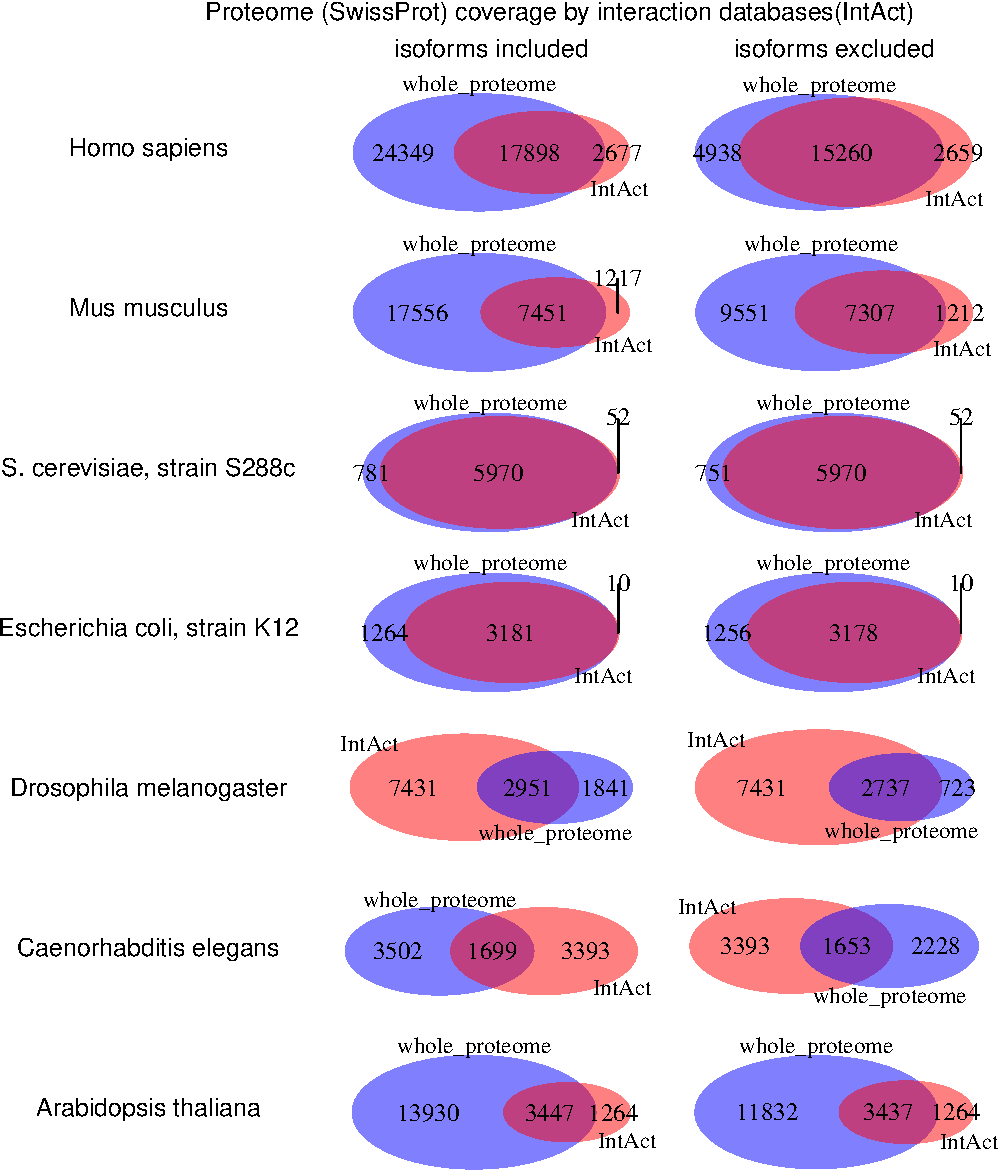
\includegraphics{final_report_text_files/figure-latex/IMEx_vs_Uniprot_venndiagram-1.pdf}
\caption{The best coverage is observed for yeast, E.coli and human.
Isoform coverage is limited, but still significant for human. Red
circles represent proteins which have interacting partners curated in
IntAct, blue circles represent proteins in SwissProt, taking into
account isoforms (left) or canonical identifiers (right).}
\end{figure}

The best interactome annotated by IMEx databases is baker's yeast, 2nd
best interactome is \emph{E.coli}. All other interactomes cover less
than the half of their respective proteome (all UniProtKB, Supplementary
figure 1). The overlap between the interactome and reviewed proteome
(SwissProt) is significantly better.\\
A large fraction of human, mouse, arabidopsis proteins and more than a
half of drosophila and \emph{C.elegans} proteins are absent in SwissProt
(but included in trEMBL) -- suggesting under-annotation by the
SwissProt-Uniprot team.\\
Protein isoforms (in multicellular model organisms) are almost not
annotated in the interactome. Human is an exception: out of 22060
protein isoforms annontated by SwissProt 2791 protein isoforms have
interacting partners. Other molecular interaction databases (active
BioGRID, inactive HPRD) do not record isoform information.

\section{2. BioGRID database (as obtained from Mentha) overlaps
significantly with IMEx
databases}\label{biogrid-database-as-obtained-from-mentha-overlaps-significantly-with-imex-databases}

BioGRID database is a major primary protein interaction database
\citep{Chatr-Aryamontri:2017aa}. IntAct and BioGRID combined contain all
interaction information which has been curated to currently active
public databases (major inactive databases include HPRD
\citep{Peri:2004aa} and BIND \citep{Isserlin:2011aa}). BioGRID uses
shallow curation level (retains only some information about the
interaction and the experiment) and identifies proteins using Entrez
Gene ID while IntAct uses UniProtKB identifiers. This has allowed
BioGRID to curate more interaction data, for example, BioGRID currently
contains interaction data from 25307 publications and compared to only
11130 in IMEx (human data only considered), more information can be
found:
\url{https://github.com/vitkl/darkspaceproject/blob/master/BioGRID/BioGRID_dsgen.md}).\\
One of the main drawbacks of BioGRID curation model is that the use of
Entrez Gene ID does not allow to distinguish between different protein
encoded by the same gene or different protein isoforms, specify
sufficient-to-bind regions of the protein. In our analysis, this
difference introduces additional identifier mapping step (Gene ID to
UniProtKB), which generates redundancy and ambiguity: several proteins
can be coded by one gene and several genes can code single proteins.
Mentha database \citep{Calderone:2013aa} has imported all BioGRID-stored
interactions and has mapped Gene ID to UniProtKB, so we used Mentha to
get BioGRID-stored interactions. Mentha doesn't import interactions for
\emph{E.coli}, therefore \emph{E.coli} is not present in this
analysis.\\
BioGRID has recently incorporated a large-scale study aimed, in part, to
find interacting partners of the proteins with no know interactions
\citep{Huttlin:2015aa}, which increases observed coverage by BioGRID.

\begin{figure}
\centering
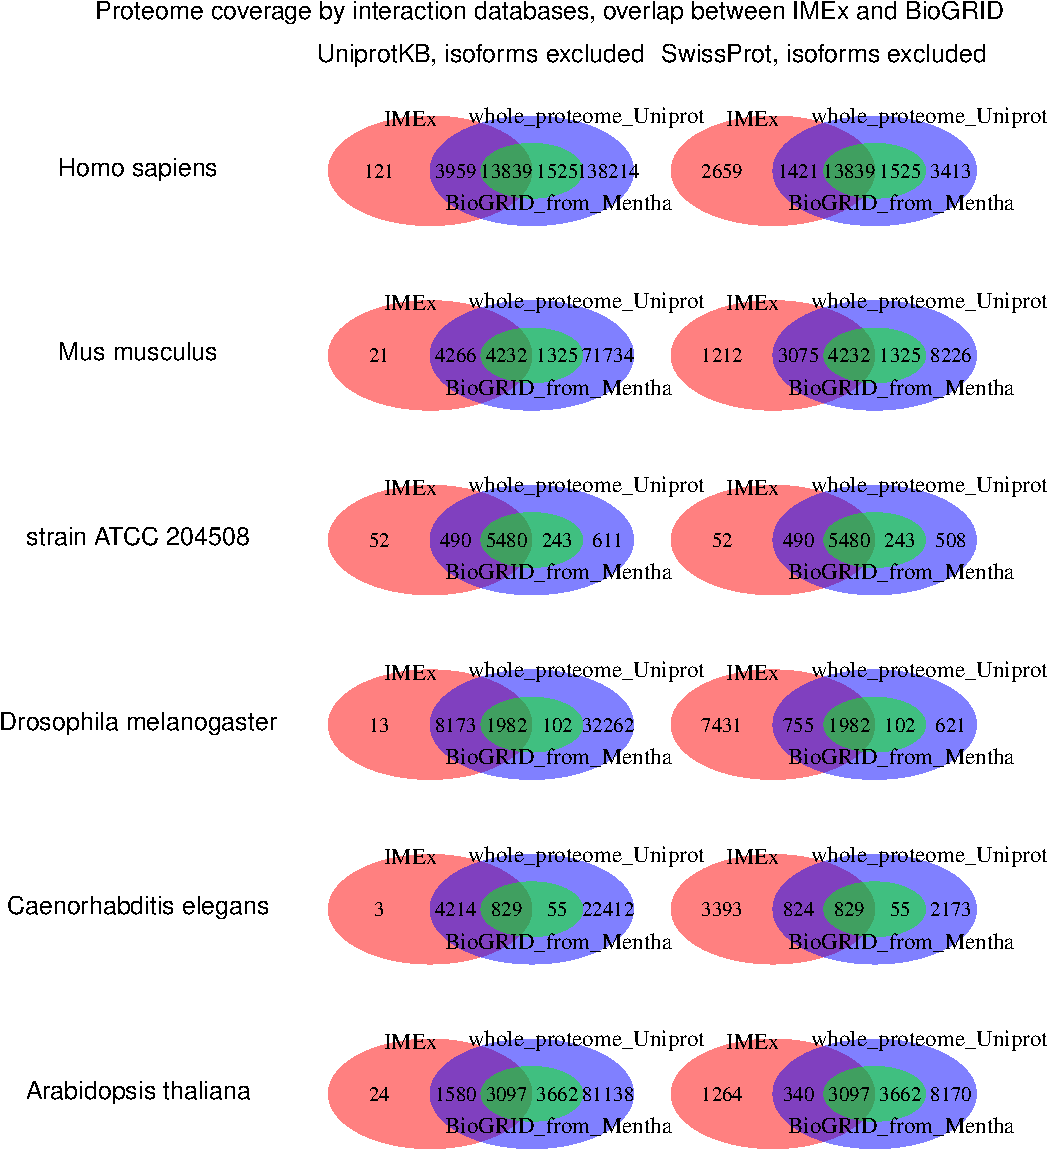
\includegraphics{final_report_text_files/figure-latex/biogrid_vs_IMEx_vs_Uniprot_venndiagram-1.pdf}
\caption{BioGRID and IMEx share a considerable fraction of proteins with
interaction data. Red circles represent proteins which have interacting
partners curated in IntAct, blue circles represent proteins in
SwissProt, green circles represent proteins which have interacting
partners curated in BioGRID, taking into account all UniProtKB (left) or
only manually reviewed SwissProt (right) proteins, only canonical
identifiers considered.}
\end{figure}

Overall, BioGRID overlaps with IMEx to a large extent. Nonetheless, for
all of the species we have looked at, BioGRID has annotated some
proteins (and their interactions) which are not annotated in IMEx.
BioGRID stores substantially more interactions for arabidopsis and a
considerable fraction of human and mouse interactions.

\section{3. Mouse and human proteins are commonly combined for
interaction
experiments}\label{mouse-and-human-proteins-are-commonly-combined-for-interaction-experiments}

The fact that researchers tend to put proteins from other species
(mostly human) into mouse experiments or tend to put mouse proteins into
cells from other species (mostly human) is also common for interaction
detection experiments and is clearly seen in Figure 7.3: half of the
mouse interactors are from the other species. This holds true both for
IMEx databases (Figure 7.3) and for BioGRID (Supplementary figure 2);
however, this analysis doesn't show which proteins (mouse or human) were
used as bait to capture interactions in which cells (mouse or human).

\begin{figure}
\centering
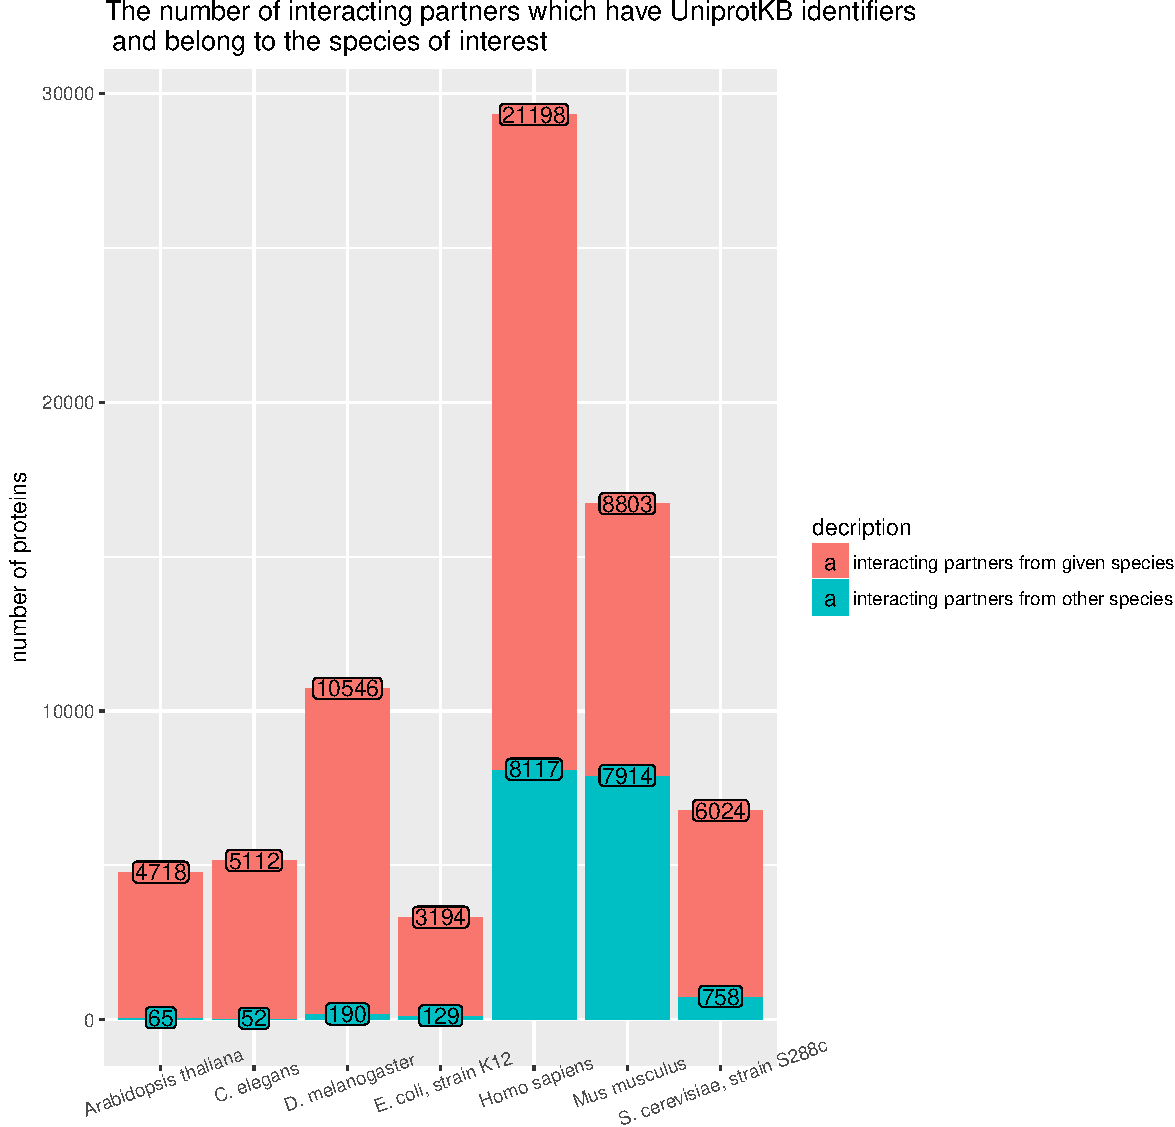
\includegraphics{final_report_text_files/figure-latex/IMEx_vs_Uniprot_N_Uniprot_Species-1.pdf}
\caption{Mouse and human proteins are commonly combined for interaction
experiments. Red bar shows the number of proteins from a given species,
blue bar shows the number of proteins from another species. Red group
proteins form interactions both with red and blue group proteins, blue
group proteins form interactions only with red group proteins}
\end{figure}

Interchangeable use of mouse and human proteins generates interaction
data which is hard to reuse and introduces imprecision due to the fact
that it requires the mapping between homologous proteins; however, this
may not be the biggest problem with studying the interactions between
mouse and human proteins and trying to correctly interpret results.
Recent studies of intrinsically disordered proteins show that linear
amino acid motifs located in disordered regions frequently mediate
protein-protein interactions \citep{Babu:2016aa}, for example, the
disordered region of p53 mediates its ability to recruit
transcription-activating proteins to the promoter \citep{Buljan:2012aa}.
More importantly, these linear amino acid motifs can evolve quickly, for
example, allowing cancer cells to escape control by P53
\citep{Buljan:2012aa}. So, while the interaction between mouse protein A
and human protein B can exist, that might not be true for the
interaction between human protein A and human protein B, and
vice-verse.\\
On the other hand, some researchers advocate that interactions important
for the cellular function should be conserved between species
\citep{Li:2017aa}.

Surprisingly, 19937 interactions between mouse and human proteins were
discovered in human rather than mouse cells (only 1510) suggesting that
researchers use mouse rather than human proteins as baits (1284 mouse
baits total, 5704 human preys total, including isoforms, from 576
publications) to find interactions directly relevant to human
interactome research, including human disease.

\section{4. Which proteins are missing interaction
evidence?}\label{which-proteins-are-missing-interaction-evidence}

Characterising the properties of proteins missing interaction evidence
can help prioritise curation efforts. By looking for proteins missing
interaction evidence and involved in particular biological function (as
described by Gene Ontology) we can complete missing part of the
interactome and decrease bias towards well-studied proteins.

\subsection{Olfactory receptors are a major group of human proteins not
represented in
IntAct}\label{olfactory-receptors-are-a-major-group-of-human-proteins-not-represented-in-intact}

We have performed Gene Ontology enrichment analysis of proteins with no
available interactions as compared to whole proteome (SwissProt protein
list). We have looked at overrepresented biological processes, molecular
fuctions and cellular compartment localisation of proteins. Here only
overrepresented biological processes are shown.

\begin{figure}
\centering
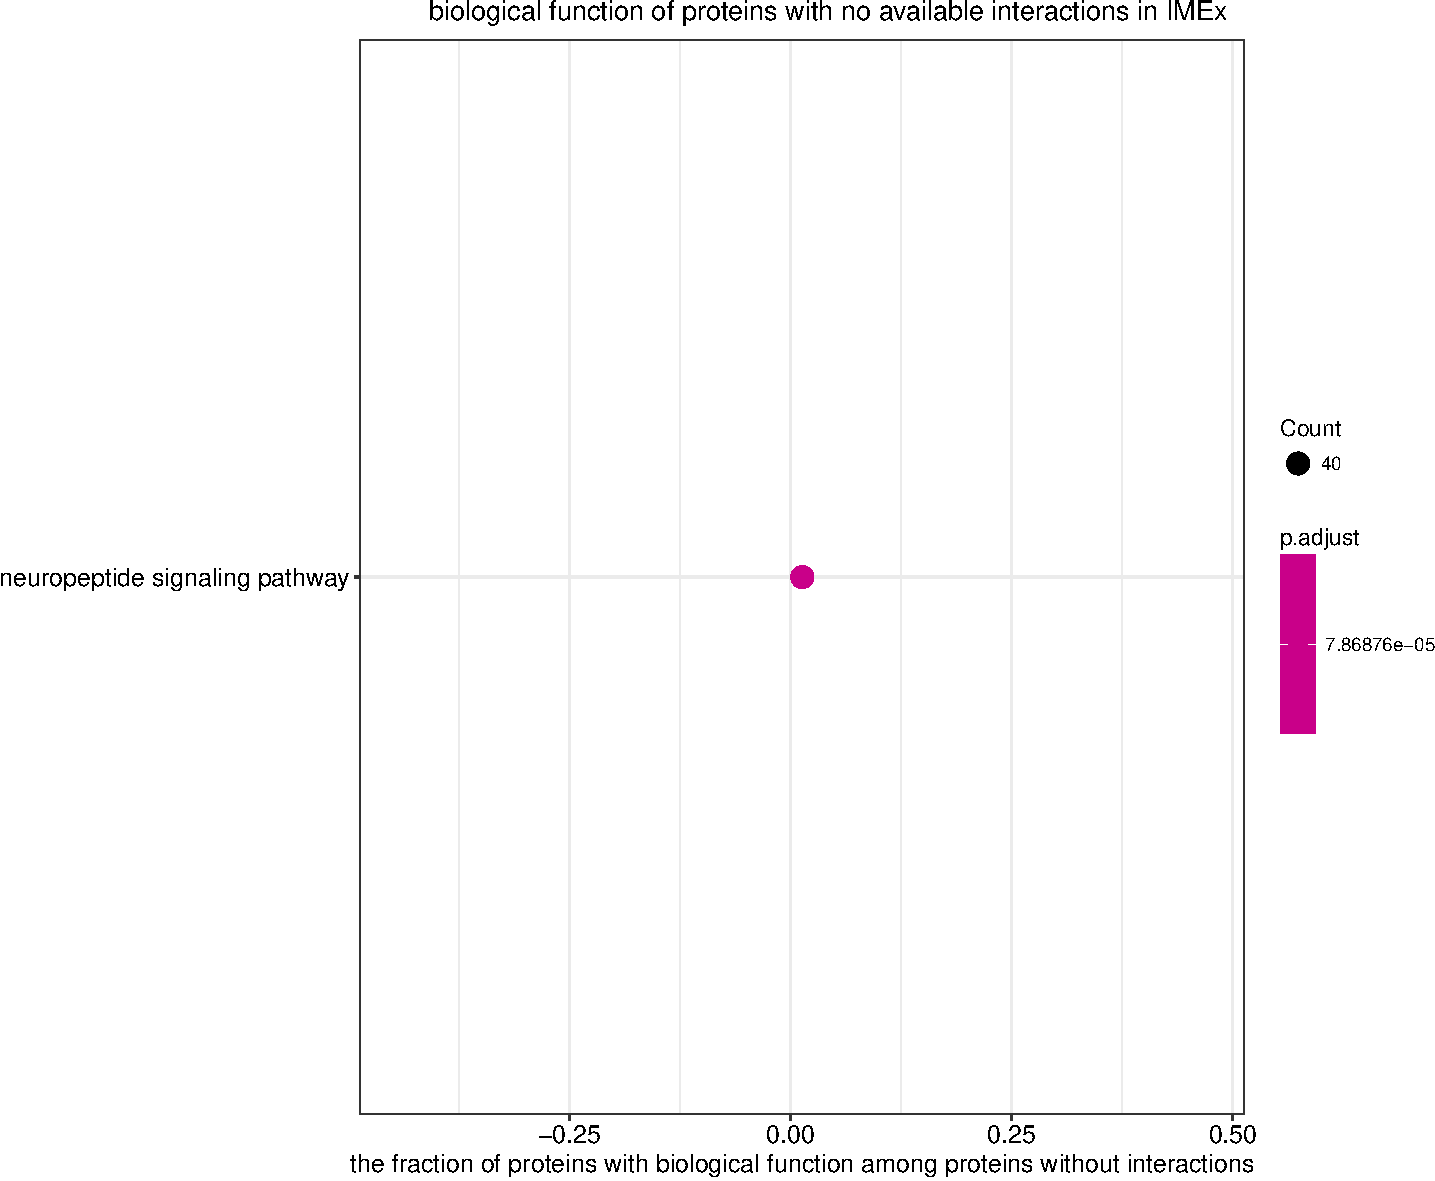
\includegraphics{final_report_text_files/figure-latex/human_not_in_IMEx_protein_properties_GO_BP-1.pdf}
\caption{Overrepresented biological processes. The size of the dot shows
the number of proteins of that category in the dataset (proteins without
interaction), x-axis represents the fraction of proteins of that
category in the dataset. Colour shows the probability of that overlap
occurring by chance.}
\end{figure}

Most of the proteins missing interactions are smell receptors, ion
channels, adhesion molecules, lipid synthesys enzymes, taste receptors.
A minor category of proteins involving sperm-egg recognition is also
overrepresented. As you might infer, all these proteins are
transmembrane or are connected to the membrane, which is also supported
by enrichment analysis for GO cellular component. We can speculate that
olfactory receptors are numerous and according to our current knowledge,
similar in function, therefore this group has not attracted enough
interest to study it's protein-protein interactions. Nonetheless,
transmembrane proteins are challenging to perform protein-protein
interactions studies on.

\subsection{Human proteins with no available interactions are on average
shorter than the proteins with interactions
available}\label{human-proteins-with-no-available-interactions-are-on-average-shorter-than-the-proteins-with-interactions-available}

Protein length or mass are physical properties of a protein which can,
in theory, influence it's usage as a bait in experiments and it's
detection in case methods depend on protein length. Proteins length is
also important biologically. Longer proteins can have multiple
functional domains and, therefore, more interactions. The distribution
of protein mass has a very long right tail - there are much more big
proteins than a normal distribution would predict (Supplementary figure
3), which only allows the use of non-parametric statistical tests
(Wilcox test is a pairwise test we have chosen). Log10 transformation of
protein mass, though, makes extreme values less extreme and is
approximately normally distributed.

\begin{figure}
\centering
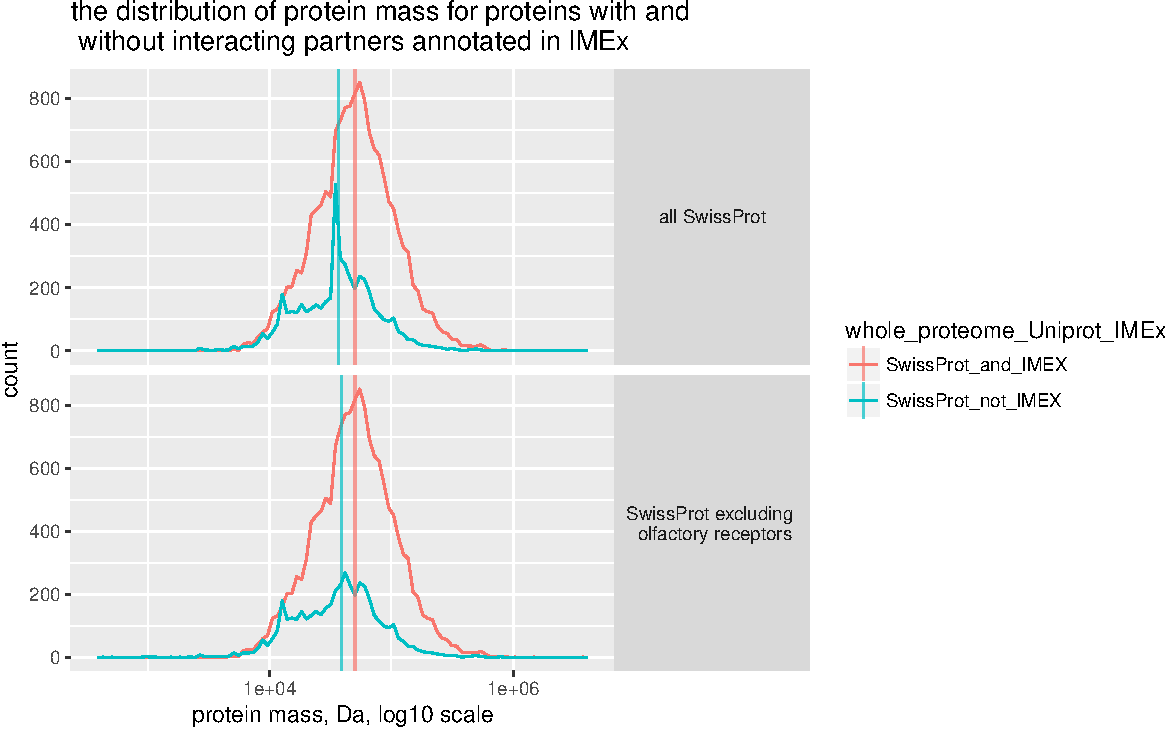
\includegraphics{final_report_text_files/figure-latex/human_not_in_IMEx_proteins_are_shorter_density-1.pdf}
\caption{Human proteins with no available interactions are on average
shorter than the proteins with interactions available. The plot compares
the distribution of protein mass across SwissProt proteins with or
without interacting partners in IntAct. Vertical line highlights the
median.}
\end{figure}

This difference in protein mass between proteins present and absent in
the interactome is highly unlikely to occur by chance (Wilcox rank test
(Mass, Da, 95\% confidence interval: -13100, -11200, p-value: 4.24e-142)
and Student t-test(log10 of Mass, Da, 95\% confidence interval: -0.154,
-0.133, p-value: 7.13e-143) on the whole population of proteins. The
removal of 416 olfactory receptors, evidently, does not change this
trend (Wilcox rank test on Mass, Da, 95\% confidence interval: -12900,
-10900, p-value: 2.14e-121).

\section{5. Do major protein interaction detection methods (two-hybrid
and AP-MS) exhibit a bias towards biochemical properties of the
proteins?}\label{do-major-protein-interaction-detection-methods-two-hybrid-and-ap-ms-exhibit-a-bias-towards-biochemical-properties-of-the-proteins}

The problem of bias in interactomics is often discussed in research
papes and in the community. Now we will focus on the bias of the
experimental detection methods. We choose to compare two major families
of methods: two-hybrid and affinity-purification followed by
mass-spectrometry (AP-MS).\\
We identify two-hybrid method using PSI-MI ontology: detection method =
``transcriptional complementation assay'' (MI:0018) - all methods which
belong to this type (which are children terms in the ontology). We
identify AP-MS method using two PSI-MI ontology terms: detection method
= ``affinity chromatography technology'' (MI:0004) and participant
identification method = ``partial identification of protein sequence''
(MI:0433). The use of ontology terms for searching interaction allows to
only specify a single term as opposed to listing every indivudual
detection method included in those groups. One can browse ontology
lookup service to identify which exact approaches are included under the
umbrella of two-hybrid or affinity-purification-mass-spectrometry.\\
We fetch interactions detected using these methods by querying molecular
interaction databases using PSICQUIC service.

\subsection{AP-MS is biased towards longer
proteins}\label{ap-ms-is-biased-towards-longer-proteins}

We have compared interaction detection method bias towards protein mass
across four species: \emph{Homo sapiens}, \emph{Mus musculus}, \emph{S.
cerevisiae} strain S288c, \emph{Escherichia coli} strain K12. We observe
that affinity-purification followed by mass-spectrometry (AP-MS) seems
to capture a higher proportion of larger proteins as compared to
two-hybrid methods. This pattern is present across four species that we
looked at, however, is manifested to a different extent. To obtain a
definitive explanation on the nature of the bias in experimental
detection method in-depth analysis of the interaction data and the
literature will be required, the goal of this study is only to identify
how the bias is manifested.

\begin{figure}
\centering
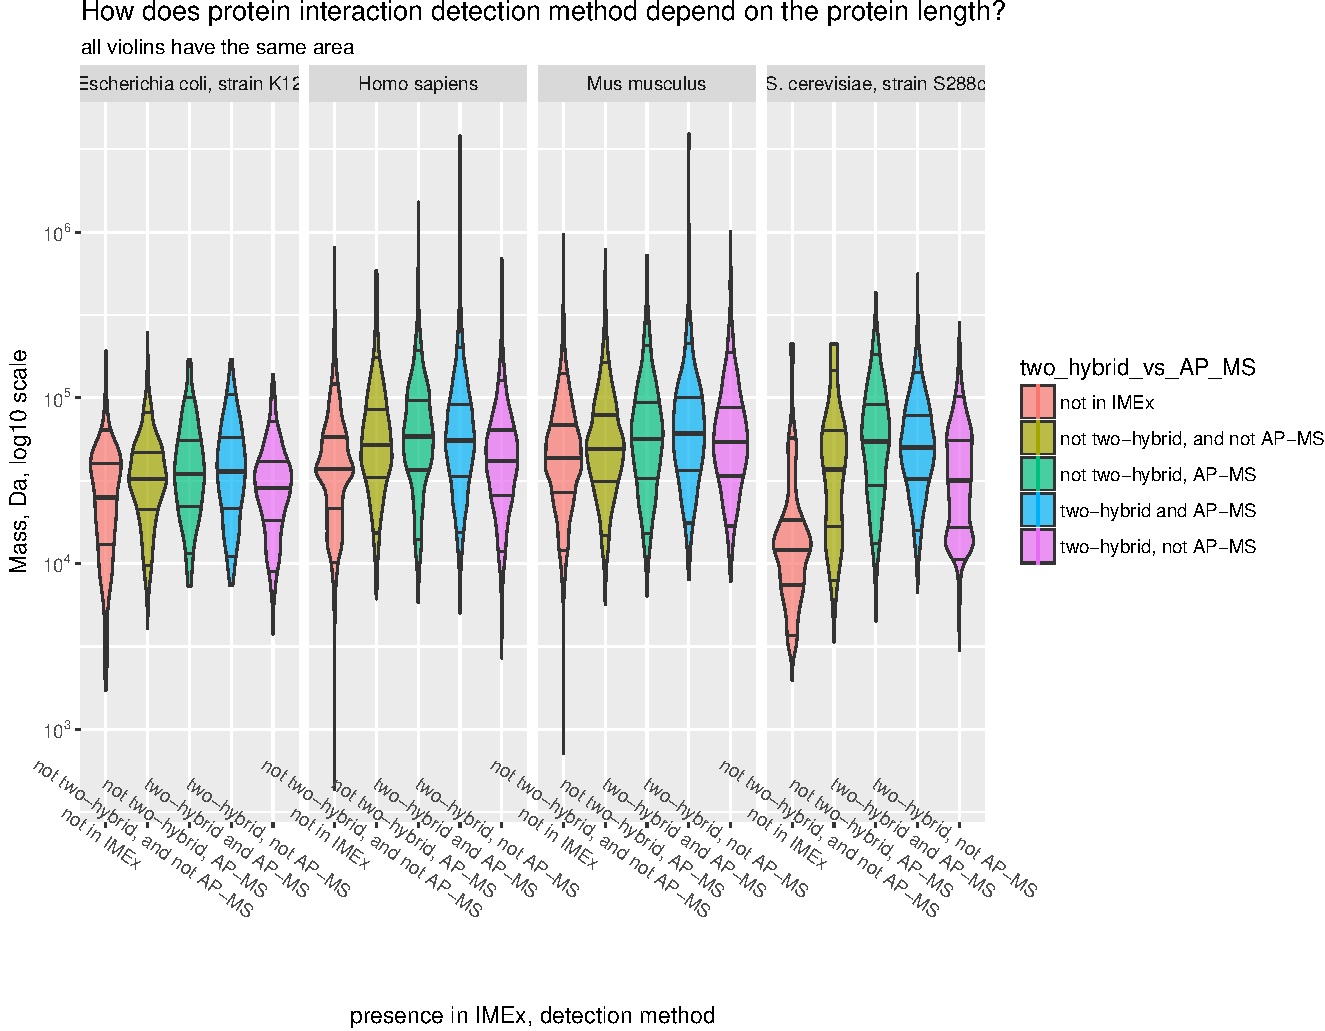
\includegraphics{final_report_text_files/figure-latex/interaction_types_combine_and_plot-1.pdf}
\caption{Plots show the distribution of protein mass across four model
species separated by interaction detection method. Details in text.}
\end{figure}

The statistical significance of the difference in protein mass across
protein detection methods was tested using linear model approach. Linear
model offers way to perform multiple statistical tests (ANOVA and
posthoc ttests) in R. Linear model takes a group assignment for a
protein (only two-hybrid, only AP-MS, both two-hybrid and AP-MS, other
methods - a vector 0s and 1s where 1 show which group a protein belongs
to) and the mass of that protein. Using these parameters for each of the
proteins linear model can learn the mean of each group as well as
provide a way to calculate errors for each of the between-group
comparisons. The robust linear model used for this test is less
sensitive to the extreme values. The figure 7.6 shows that the mass of
the proteins which were identified interacting using AP-MS technique is
on average higher that the mass of the proteins identified using
two-hybrid or the other methods.

\subsection{Major experimental role types (bait/prey/neutral component)
are influenced by the mass of the protein in two-hybrid
assays}\label{major-experimental-role-types-baitpreyneutral-component-are-influenced-by-the-mass-of-the-protein-in-two-hybrid-assays}

The experimental role of the protein (bait/prey/neutral component) can,
in theory, be influenced by protein mass. For example, it may be easier
to clone shorter proteins for use as bait/prey. So it important to see
if the experimental role is really influenced by protein mass. We also
factor in the interaction detection method.

\begin{figure}
\centering
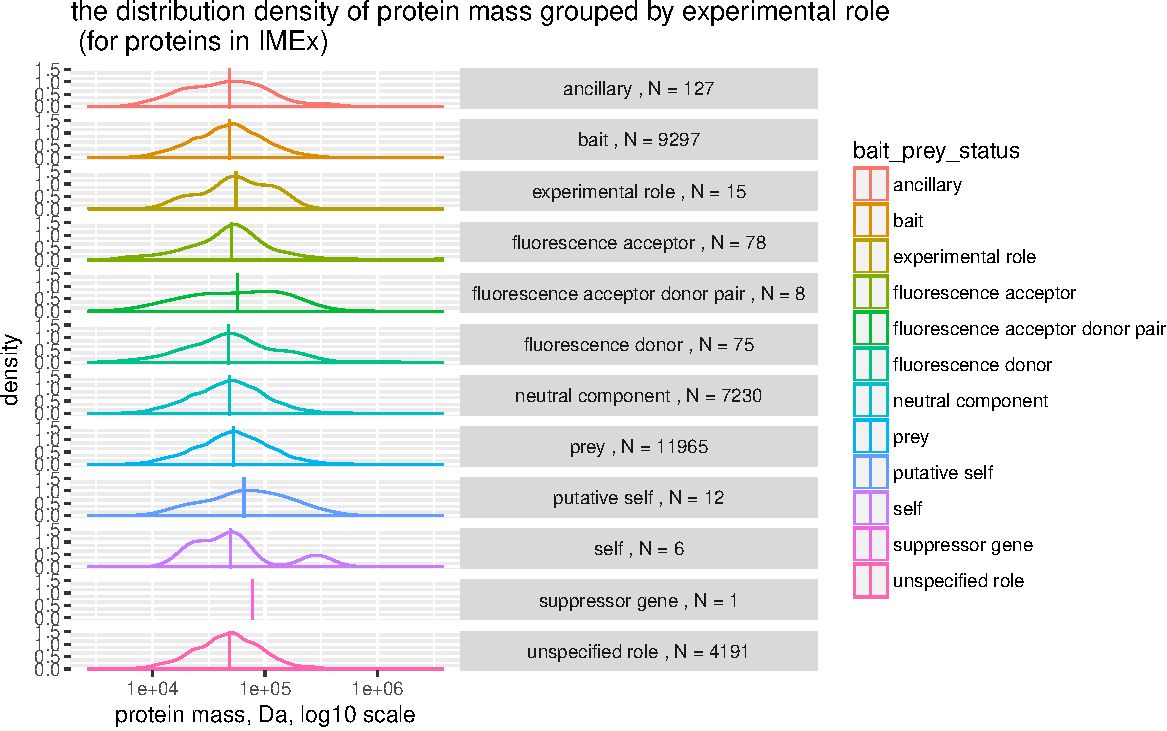
\includegraphics{final_report_text_files/figure-latex/human_not_in_IMEx_bait_vs_non_bait-1.pdf}
\caption{Experimental role of a protein, such as bait or prey, is
influenced by the mass of the protein in two-hybrid assays. Due to no
fundamental distinction between the bain and the prey in these assays
the result may be reflective of the experiment setup. The area of the
violin corresponds the number of observation in each group (legend on
the left). ``not two-hybrid, AP-MS'' tab clearly show that AP-MS
techniques identify many preys per single bait (the issue was discussed
in the introduction).}
\end{figure}

Evidently, the experimental role of a protein is influenced by the
protein length in two-hybrid methods: prey proteins tend to be longer
than bait proteins. Two hybrid bait and prey are not fundamentally
different. In two-hybrid methods, bait protein and prey protein can be
cloned into either of the plasmids used in the assay, in contrast, AP-MS
aproaches use antibodies targeting the bait to purify the bait and any
protein interacting with it, this way, pray proteins don't need to be
cloned the assay to work, now cloning restriction applies. So the
distinction observed is not descriptiptive of protein as much as it is
of the experimental setup. Potential explanation might be that fragments
of proteins (aimed to identify sufficient to bind regions) are often
cloned as a bait. This bias might also be created by a specific
high-throughput two-hybrid study.

\chapter{Conclusions}\label{conclusions}

Our analysis shows that main model species have interaction data for the
substantial fraction of the proteome. It also suggests that interaction
data is still biased \citep{Rolland:2014aa} towards well-researched
proteins. We can also see that interaction detection methods have
specific biases; however, we were don't see many of the effects from the
original study on structural bias published 8 years
ago\citep{Bjorklund:2008aa}. The latter supports the take-home-message
of that paper: aggregated datasets of protein interactions represent a
more robust source for drawing conclusions. Large fraction of IntAct
proteins are also present in BioGRID which combined with the result of
functional enrichment suggest that the bias we see in the coverage comes
the fact that some categories proteins are underresearched and not from
the undercuration by IntAct or BioGRID teams. Finally, our result
suggests that all experimental resources (human interaction data only)
have similar bias to biological process, molecular function or the
cellular localisation of the proteins; however, STRING database, which
includes computational prediction data, is the least biased.\\
Result of this study have served as a foundation to a data integration
project aimed use multiple protein-protein interaction resources and
machine learning to find publications which contain protein-protein
interactions not yet curated into IntAct database. This project has a
potential to reduce bias in the interaction data, increase accessibility
of currectly published protein-protein interactions involving proteins
with underrepresented functions and in currently in progress
\citep{PPorras2017}.

\chapter{Supplementary figures}\label{supplementary-figures}

\section{Supplementary figure 1}\label{supplementary-figure-1}

\begin{figure}
\centering
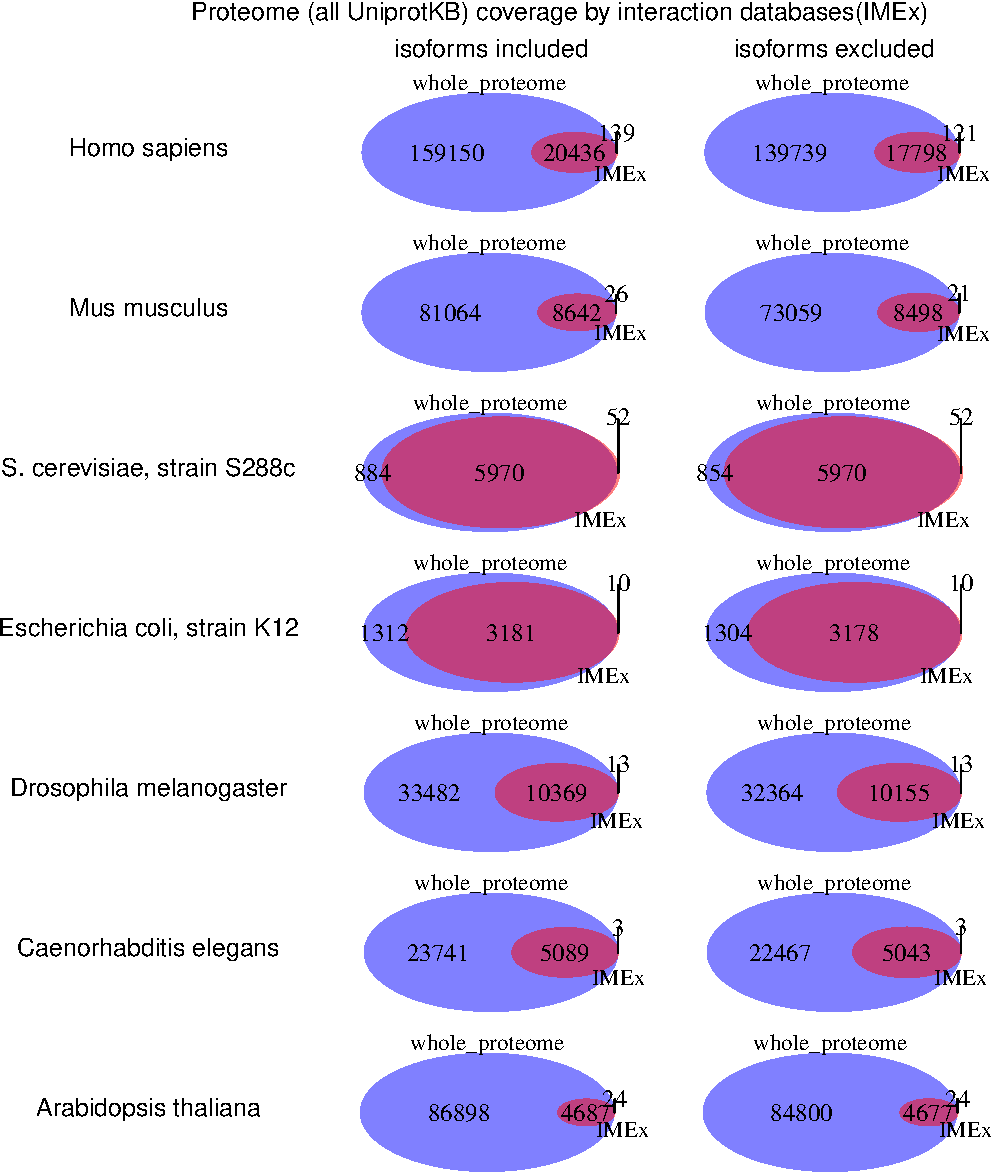
\includegraphics{final_report_text_files/figure-latex/Supplementary1_IMEx_vs_Uniprot_venndiagram_all_Uniprot-1.pdf}
\caption{Supplementary figure 1. The overlap between proteins with known
interactions (interactome) and all proteins included in UniprotKB
(proteome). Red circles represent proteins which have interacting
partners curated in IntAct, blue circles represent proteins in
SwissProt, taking into account isoforms (left) or canonical identifiers
(right).}
\end{figure}

\section{Supplementary figure 2}\label{supplementary-figure-2}

\begin{figure}
\centering
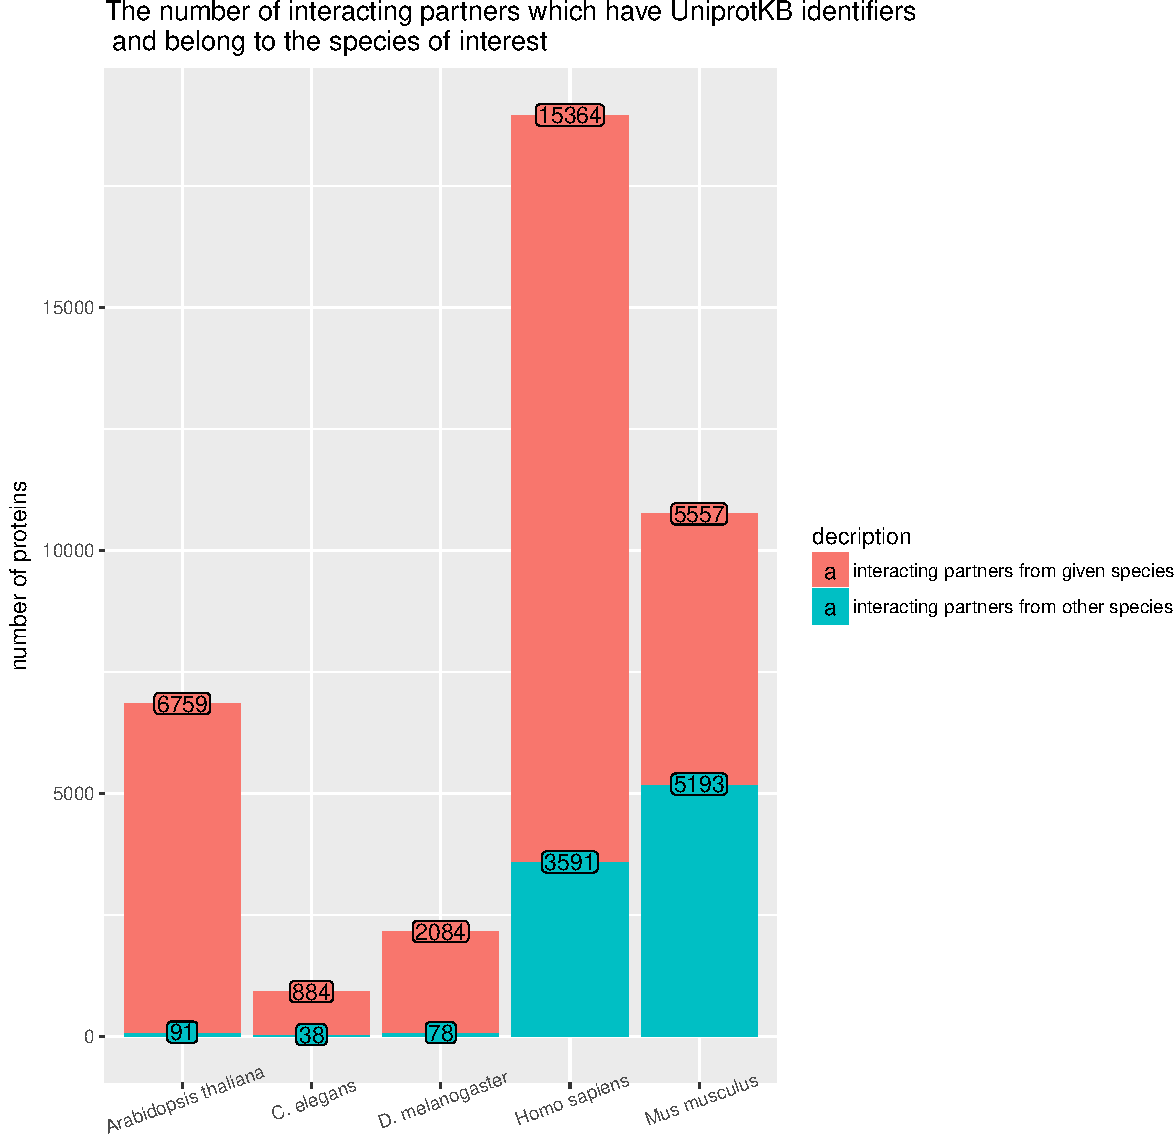
\includegraphics{final_report_text_files/figure-latex/Supplementary2_BioGRID_vs_IMEx_vs_Uniprot_N_Uniprot_Species-1.pdf}
\caption{Supplementary figure 2. The number of interacting proteins from
given species or the other species in BioGRID. Red bar shows the number
of proteins from a given species, blue bar shows the number of proteins
from another species. Red group proteins form interactions both with red
and blue group proteins, blue group proteins form interactions only with
red group proteins.}
\end{figure}

\section{Supplementary figure 3}\label{supplementary-figure-3}

\begin{figure}
\centering
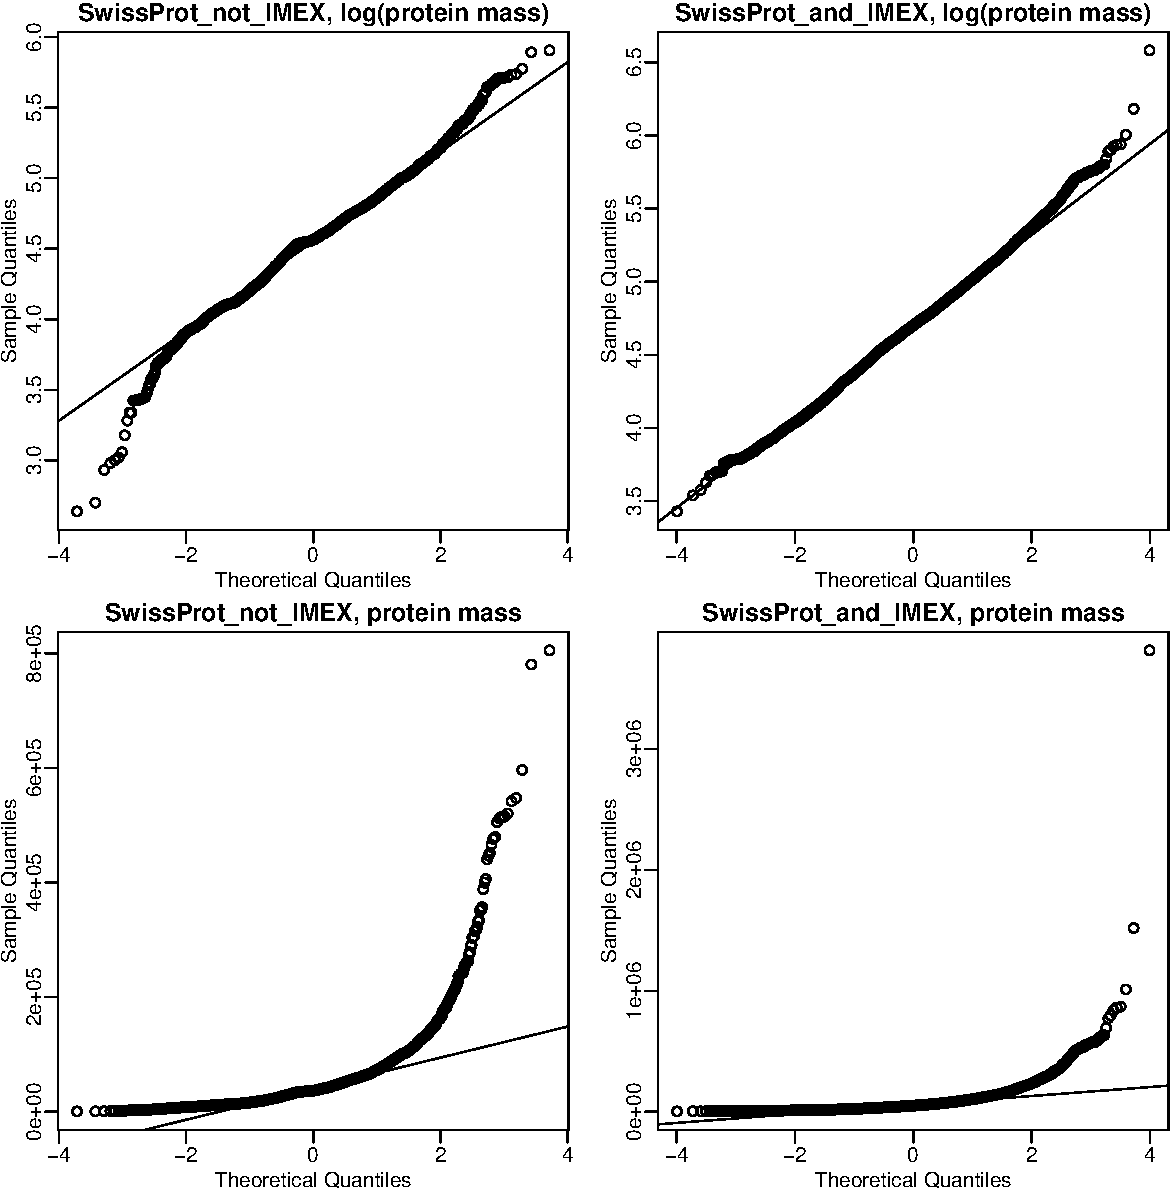
\includegraphics{final_report_text_files/figure-latex/Supplementary3_protein_mass_distribution_qqplot-1.pdf}
\caption{Supplementary figure 3. Proteomes have much more long proteins
than normal distribution would predict (proteins, dots, are above the
line in qq-plot). The distribution of logarhithm base 10 of protein mass
is approximately normal. In this plot the distribution of the data is
plotted against the normal distribution. If dots fall below the curve of
the left or above the curve on the right this would suggest that normal
distribution underpredict the number of extreme values which will skew
the result of parametric statistical test.}
\end{figure}

\section{Supplementary figure 4}\label{supplementary-figure-4}

\begin{figure}
\centering
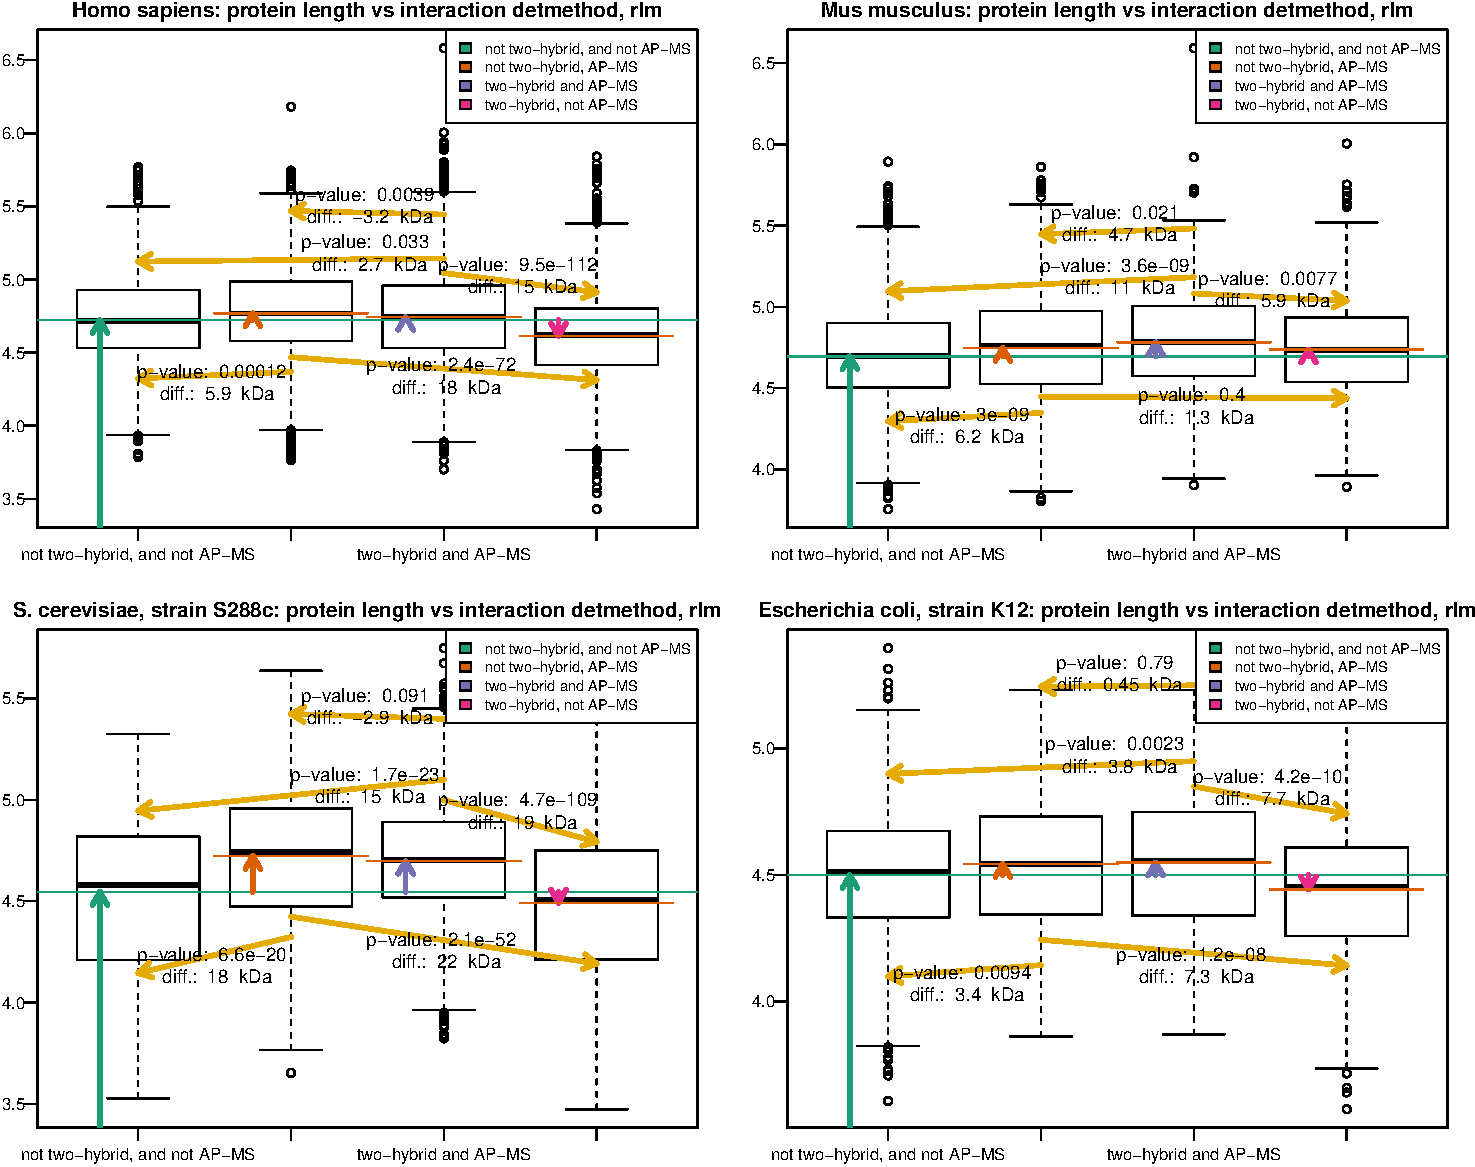
\includegraphics{final_report_text_files/figure-latex/protein_length_det_method_rlm-1.pdf}
\caption{Supplementary figure 4. The results of statistical tests can be
visualised on a plot. In the box plot below, each vertical arrow points
to the median mass of the proteins in a particular group. The middle
line of the boxplot represents a median which happens to coincide with
mean because the distribution of logarithm base 10 of mass is
approximately normally distributed. Each yellow arrow shows the p-value
and the difference in protein mass between two corresponding groups.}
\end{figure}

\bibliography{bibtex_library.bib}


\end{document}
